% arara: pdflatex: {options: "-draftmode"}
% arara: biber
% arara: pdflatex: {options: "-draftmode"}
% arara: pdflatex: {options: "-file-line-error-style"}
\documentclass[MilwayThesis]{subfiles}
\begin{document}

This dissertation rests on a number of non-standard theoretical assumptions and draws a few non-standard distinctions, which I will defend in this chapter.
My defense of the assumptions, however, will not be an argument that they are true, as the truth of any theoretical statement ultimately depends on the empirical facts.
Rather, my defense will actually be an offense; I will argue that the standard assumption is, in fact, ill-founded.
So, in a sense, I will be rejecting standard assumptions rather than making non-standard ones.
The distinctions I draw, in contrast, will not be defended, but rather explained and clarified.

\section{The $\Theta$-Criterion}
The $\theta$-criterion standardly assumed was first formulated by Chomsky in \textit{Lectures in Government and Binding} (LGB) as \Next.
\ex. Each argument bears one and only one $\theta$-role, and each $\theta$-role is assigned to one and only one argument. \parencite[36]{chomsky1981lectures}

In a footnote, Chomsky justifies this criterion, saying 
\begin{quote}
	The second clause of [the $\theta$-criterion] is well-motivated.
	To say that each $\theta$-role must be filled implies, for example, that a pure transitive verb such as \textit{hit} must have an object, that a verb such as \textit{put} or \textit{keep} (with the sense they have in \textit{put it in the corner}, \textit{keep it in the garage}) must have the associated PP slot filled, etc. 
	The additional requirement that each $\theta$-role must be filled by only one argument will, for example, exclude the possibility that a single trace is associated with several argument antecedents, a possibility ruled out in principle under the Move-$\alpha$ theory. 
	\parencite[139]{chomsky1981lectures}
\end{quote}
I would agree that the second clause of \Last, that each $\theta$-role is assigned to a single argument, is well-motivated by the empirical considerations Chomsky cites, and as such I will not reject that portion of the $\theta$-criterion.
The first clause, however, is motivated mainly by theoretical concerns of LGB, that is, its connection to empirical facts is indirect at best.

The nature of the LGB theory is such that its various hypotheses and principles are connected to each other in a web-like network.
As a result, the first clause of the $\theta$-criterion depends on various other theoretical statements and various other theoretical statements depend on it.
So, rather than attempting an exhaustive enumeration of the links between the $\theta$-criterion and the other theoretical statements of LGB, I will present what I consider to be the best argument in favour or the $\theta$-criterion, and argue that its premises have since been rejected within syntactic theory.

The first premise is the now familiar Y- or T-model of grammar shown in \Next, which LGB theory continues from earlier theories.
According to this model, a syntactic derivation has four levels of representation (D-structure, S-Structure, PF, and LF), and each step in the derivation is performed by the application of a subset of the transformational rules.
S-structures are derived by the applying of Move-$\alpha$ to D-structures, LFs are derived by applying QR (and maybe Move-$\alpha$) to S-structures, and PFs are derived by applying ``stylistic rules'' to S-structures \parencite[18]{chomsky1981lectures}.
\ex. 
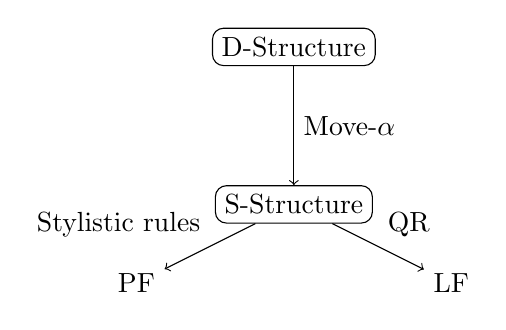
\begin{tikzpicture}[baseline]
	\node[draw,rounded corners] (DS) at (0,0) {D-Structure};
	\node[draw,rounded corners] (SS) at (0,-2) {S-Structure};
	\node (PF) at (-2,-3) {PF};
	\node (LF) at (2,-3) {LF};
	\draw[->] (DS)--(SS) node[midway,right] {Move-$\alpha$};
	\draw[->] (SS)--(PF) node[midway,anchor=south east] {Stylistic rules};
	\draw[->] (SS)--(LF) node[midway,anchor=south west] {QR};
\end{tikzpicture}

The exact natures of the transformations are not important for this discussion.
What is important, is that all syntactic displacement is the result of one of these transformations.

The second premise is the projection principle, which states that lexical properties must be represented at all levels of syntax.
Since $\theta$-roles are lexical properties of (at least) verbs, they must be represented at all levels of syntax.
Consider the verb \textit{hit}, whose lexical entry specifies that it needs a patient argument.
The projection principle requires that at D-Structure and S-Structure \textit{hit} must have assigned a patient $\theta$-role to an argument and therefore, assuming the patient $\theta$-role is assigned to Comp,V, there must be a DP in the complement position of \textit{hit} at both D-Structure and S-Structure.

With these assumptions, it follows that no single argument can receive more than one $\theta$-role.
Suppose there is a derivation in which a single argument X receives two $\theta$-roles $\Theta1$ and $\Theta2$.
According to the projection principle, X must be marked with both $\Theta1$ and $\Theta2$ at D-Structure.
Since each $\theta$-role is associated with a unique structural position, it follows that X must be in two distinct positions at D-Structure.
The only way an argument can be in mutiple positions is if it has undergone Move-$\alpha$.
Move-$\alpha$, however, maps D-Structures to S-Structures.
Therefore, an argument cannot be in two positions at D-Structure, and futhermore, cannot be multiply $\theta$-marked at D-Structure.
If an argument cannot be multiply $\theta$-marked at D-Structure, then it cannot be multiply $\theta$-marked at all.

Thus we are able to derive the first clause of the $\theta$-criterion from other principles.
These principles, however, have either been rejected or problematized since their statement in LGB.
Since \textit{The Minimalist Program} \parencite{chomsky1995minimalist}, generative theories have largely dispensed with D-Structure and S-Structure.
Without these levels of representation, the projection principle (as formulated in LGB) is effectively meaningless, and without the projection principle, there is no more basis for the first clause of the $\theta$-criterion.
Therefore, I will not be assuming the first clause of the $\theta$-criterion.

\section{Last Resort}

\end{document}
